\chapter{Preprocessing image}
Preprocessing image is the process that reduces the noises or removes unexpected objects from image. Preprocessing image is used to enhance the quality of input dataset (images) when doing a test of an algorithm or a method. Following the requirement, we apply one or more operations to pre-process images. In this chapter, we discuss about a method to pre-process images we applied in this internship. The method is suggested based on the basic knowledge the operations in image processing.
\section{Problem}
With the input dataset is a set of 293 insect images. Each image contains the body parts of insect(body, head,...) and an unexpected object, specifically yellow grid (figure \ref{fig:figure_31}). To enhance the accuracy of the classify method, we need to remove the grid and just keep the insect on each input image.
\begin{figure}[h!]
\centering
\subfloat[The yellow gird on the left of insect]{\label{fig:example_1}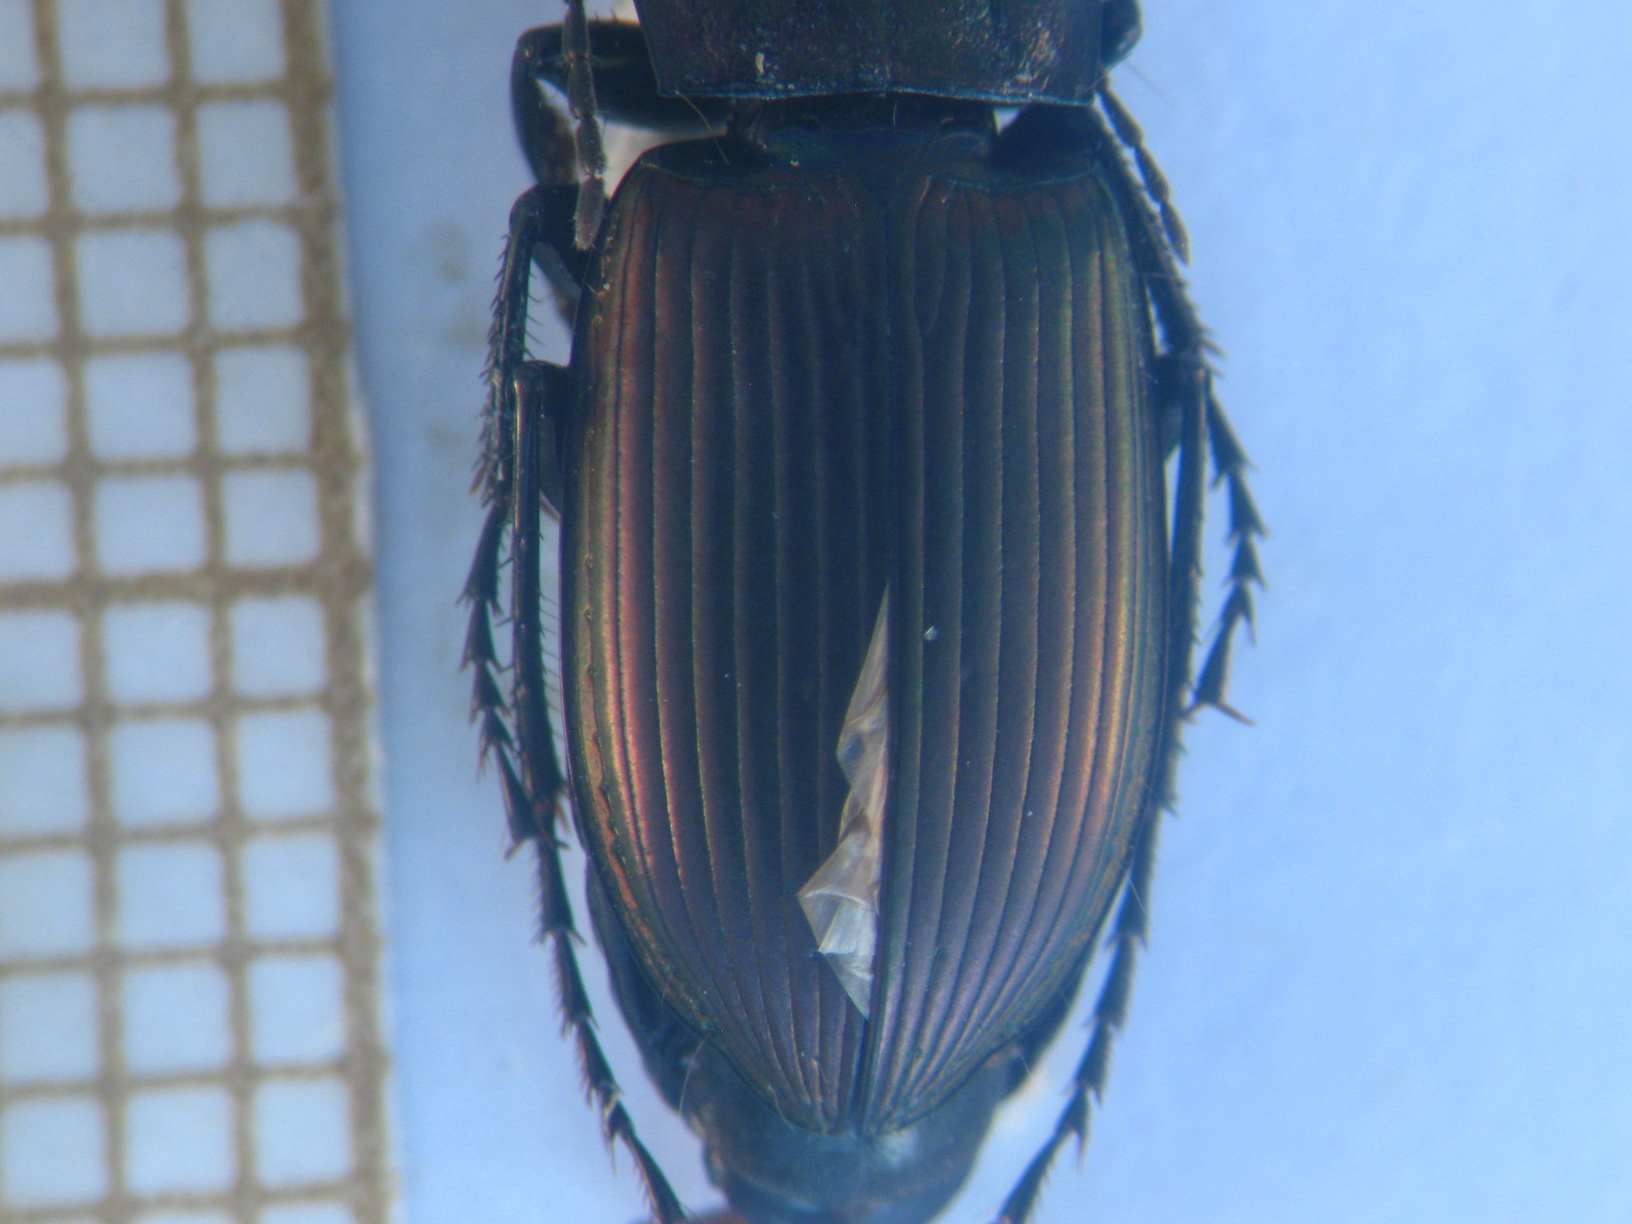
\includegraphics[width=0.4\textwidth]{./images/input1}}~~
\subfloat[The insect overlap the yellow grid]{\label{fig:example_2}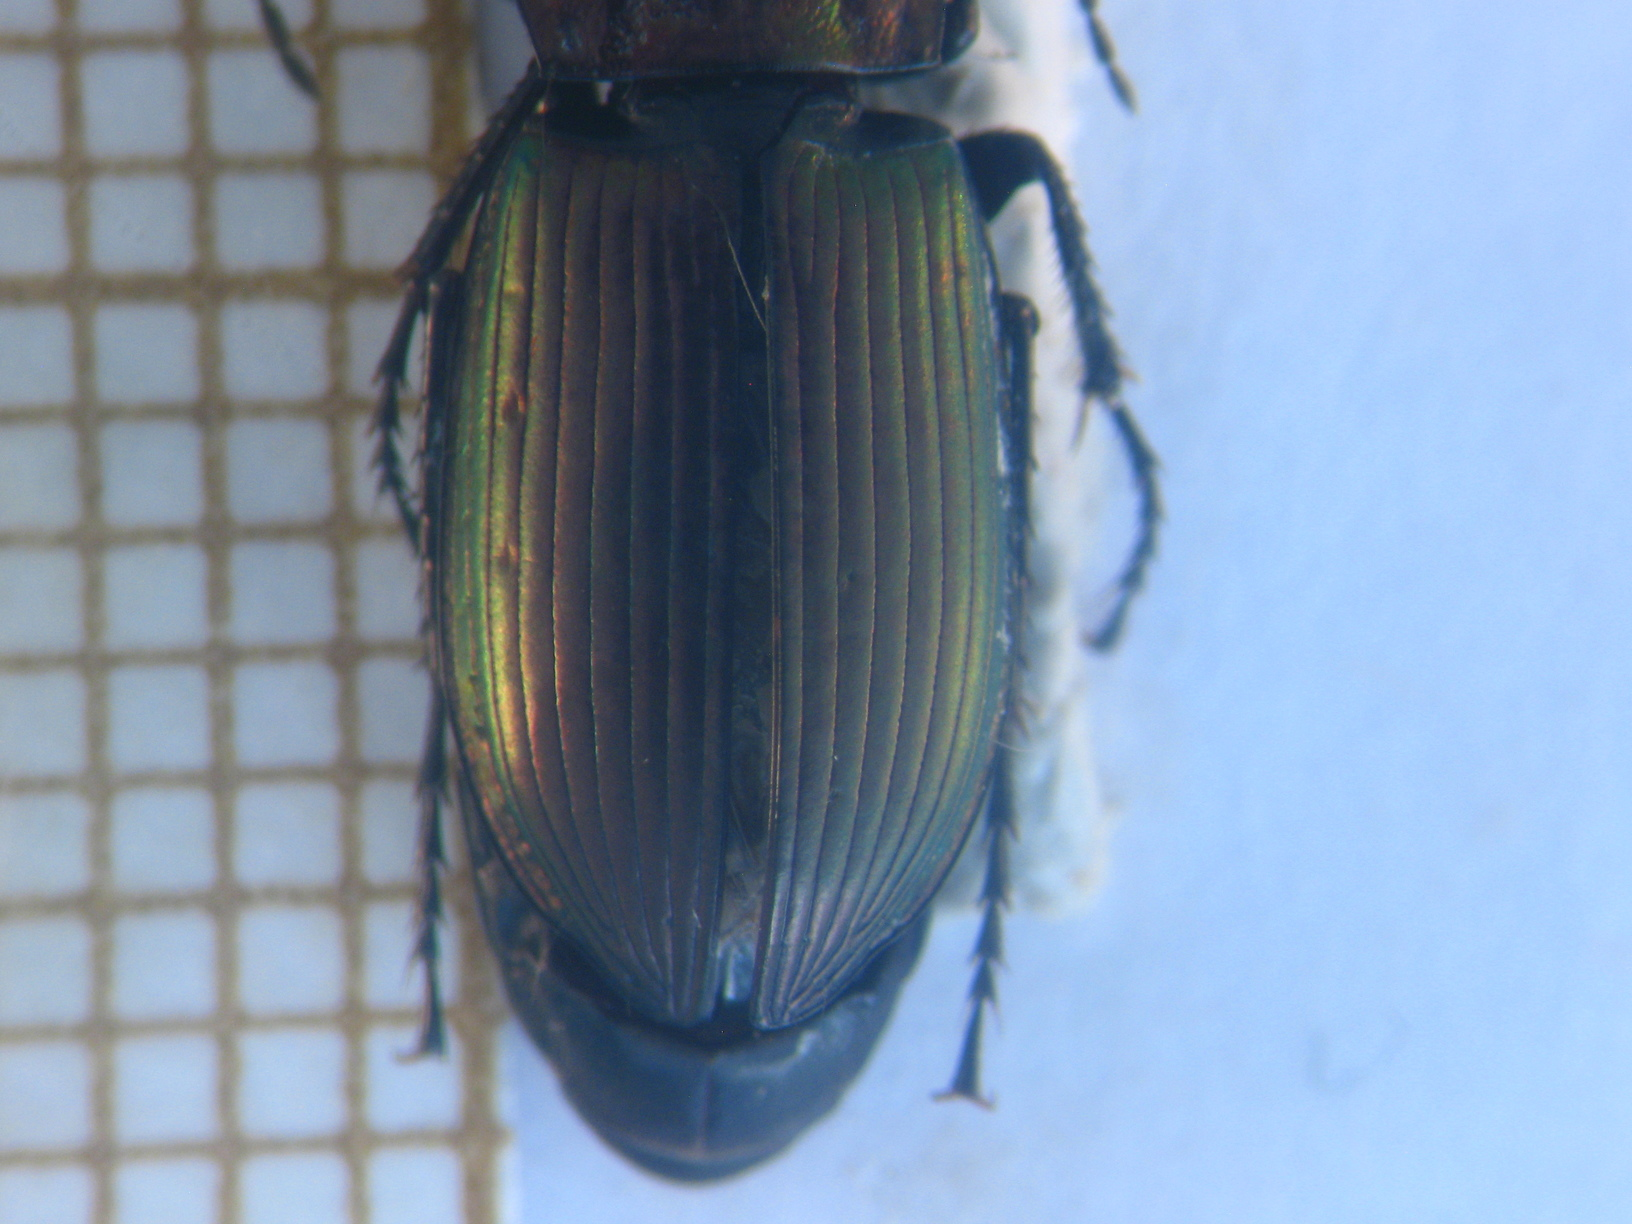
\includegraphics[width=0.4\textwidth]{./images/input2}}
\caption{The input images with yellow grid}
\label{fig:figure_31}
\end{figure}
\section{Analysis}
Each input image contains two objects: a part of an insect (named insect) and the yellow grid (named grid). About the relative position, the grid always stayed on the left of an insect, and the insect may overlap the grid. About the color, images are presented in BGR model with three main color groups: the background color, the yellow color of grid and the color of the insect.\\[0.2cm]
The method proposed to remove the grid based on the color processing. If we process the image in BGR model, the algorithm may be complex because the color at each pixel is combined of three values (blue, green, red). Because HSV model has a specific channel to present the colors with clear range we can apply this property for detecting and removing the gird. The proposed process removes the grid as follows:
\begin{enumerate}
\item Find the ``\textit{limit}" points of the grid: the points stay nearest outside grid.
\item Find the ``\textit{replace}" points:  the location that its value is used to replace to the grid.
\item Replace the grid by the value of ``\textit{replace}" point.
\end{enumerate}
\subsection{Find the limit and the replace points}
Browsing image to check and replace the pixels in gird needs a long time. To reduce the time complexity, we should find the limit range of the grid. The limit of the gird is defined by the points located out of the gird and its closest. Instead of checking all pixels, we check the pixels stay on the left of the limit points. The idea is to find the limiting point outside of grid is finding a column that the number of \textit{yellow} points stays on this column keep in permitted level.\\
Because the grid always stays on the left land side of the image and the ``width" of the grid usually less than two-thirds of the width of the whole image. So, to reduce time complexity, we check from the beginning of the image to two-thirds of image. The result of this step is the limit points, these points will be used to limiting the length when we check the pixels on yellow grid.\\
\textbf{The algorithm to find the limit points are as follows:}\\
\begin{algorithm}[H]
\Indm
\KwData{$inputImage$: The input image (contains the insect and grid)}
\KwResult{The coordinate of limit point}
\Indp
Declare some variables: $Mat$ $hsvImage$; $vector<Mat> hsv\_channel$\;
Convert image from BGR to HSV: $cv:cvtColor(inputImage, hsvImage, COLOR\_BGR2HSV)$ \;
Split HSV image into several channel: $cv::split(hsvImage, hsv\_channels)$\;
Set up initial \textit{limit\_point} and assign with the left-top corner: 
$Point$ $limit\_point = Point(0,0)$\;
Declare a variable $yellow\_count$ to count the number yellow points on each columns when processing.\;
\For{$j \leftarrow 10 $ \KwTo $image\_width * 2/3$}{
	\If{H value at $(5,j) > $ 100 \textbar \textbar (H  value at $(5,j) > 70$ $\&\&$ H value at $(5,j) < 100$\\
				$\&\&$ S value at $(5,j) < 10 $ $\&\&$ V value at $(5,j) > 175$ )
		}{
		$limit\_point.x \leftarrow j$\;
		$limit\_point.y \leftarrow 0$\;
		$yellow\_count \leftarrow 0 $\; 
		\For{$i \leftarrow 1 $ \KwTo $hsv\_channel[0].rows * 2/3$}{
			\If{H value at $(i,j) <= 38 $}{
				$yellow\_count++$\;
				\If{$yellow\_count >= 8$}{
					$limit\_point.x \leftarrow 0$\;
					$limit\_point.y \leftarrow 0$\;		
					break\;	
				}		
			}
		}
		\If{$limit\_point.x != 0$}{
			break\;
		}
	}
}
\If{$limit\_point.x == 0$}{
	$limit\_point.x \leftarrow hsv\_channel[0].columns/3 + 200$\;
	$limit\_point.y \leftarrow 0$\;	
}
\caption{Algorithm to find the limiting points}
\end{algorithm}~~\\
Now, we indicate what is the color that used to replace the yellow points. Hence, we choose the points having the value nearest with the background color. The histogram is ideal in choosing the position to replace, but we have rules to obtain a good value.\\
The algorithm to find the replacing points are as follows:\\
\IncMargin{1em}
\begin{algorithm}[H]
\Indm 
\KwData{inputImage: the input image}
\KwResult{The coordinate of replacing point}
\Indp
Convert image to gray scale image\;
Calculate the histogram on gray scale image and mean of histogram\;
Split the HSV image into channels\;
\For{$i \leftarrow 0 $ \KwTo $grayImage.rows$}{
		\For{$j \leftarrow 0 $ \KwTo $grayImage.columns$}{
		\If{value at $(i,j) > $mean of histogram\\
			$\&\&$ H value (i,j) $>$ 90\\
			$\&\&$ H value (i,j) $>$ 130\\
			$\&\&$ S value at (i,j) $>$ 50\\
			$\&\&$ V value at (i,j) $>$ 215 }{
			return this position \;
		}
	}
}

\caption{Algorithm to find the replacing point}
\end{algorithm}\DecMargin{1em}
\subsection{Replacing the grid}
The grid does not contain only the yellow points. It also contains the points which have the similar color with the backgrounds but the brightness is difference (called \textit{miss bright} points). Thus, replacing the gird means to replace both the yellow and the \textit{miss bright} points.\\
After having the limit and the replace point, we replace the grid by processing on all rows of image. On each row, we replace the value at each pixel by the value at replace point. This works repeatedly until meeting the limit points or a ``special point" (called ``break" point). It can be a point stays on the insect or a point belongs to the background.\\
For each part of the insect, the color of the insect or the background also have the different values. Thus, we need to define the different special value (break point) for each parts based on the file name of the image.\\
\IncMargin{1em}
\begin{algorithm}[H]
\Indm
\KwData{filePath: the file path of image}
\KwResult{Which part of insect in image}
\Indp
\textit{QString} temp $\leftarrow$ filePath.toLower()\;
\If{temp contains ``ely"}{
	return ELYTRE\;
}
\If{temp contains ``md"}{
	return MDROITE\;
}
\If{temp contains ``mg"}{
	return MGAUCHE\;
}
\If{temp contains ``prono"}{
	return PRONOTUM\;
}
\If{temp contains ``tete"}{
	return TETE\;
}
return ELYTRE\;
\caption{Algorithm to get the parts of insect}
\end{algorithm}
\DecMargin{1em}
\IncMargin{1em}
\begin{algorithm}[H]
\Indm
\KwData{inputImage: the input image; limit\_point: the limit point; part: part of insect; minBrightness: minimum of brightness; rpoint: replacing point}
\KwResult{The image after replace the yellow grid}
\Indp
\For{$i \leftarrow 0 $ \KwTo $inputImage.rows$}{
		\For{$j \leftarrow 0 $ \KwTo $limit\_point.x$}{
		\If{part is ELYTRE}{
			\If{ value at $(i,j+50)$ satisfy breaking condition}{
				break\;
			}
		}
		\If{part is MDROITE or MGAUCHE}{
			\If{ value at $(i,j+50)$ satisfy breaking condition}{
				break\;
			}
		}
		\If{part is PRONOTUM}{
			\If{ value at $(i,j+50)$ satisfy breaking condition}{
				break\;
			}
		}
		\If{part is TETE}{
			\If{ value at $(i,j+50)$ satisfy breaking condition}{
				break\;
			}
		}
		\If{H value at $(i,j+50)$ in yellow range}{
			replace value at this point by the value at replacing point\;
		}\lElse{
			\If{V at $(i,j+50) > $ minBrightness}{
				replace value at this point by the value at replacing point\;
			}
		}
	}
}
Merging three channel of HSV\;
Convert the image from HSV to BGR\;
\caption{Algorithm to replace the yellow grid}
\end{algorithm}
\DecMargin{1em}







































